\documentclass[a4paper,11pt]{article}
\usepackage{amsmath,amsthm,amssymb}
\usepackage[utf8]{inputenc}
\usepackage[english,russian]{babel}
\usepackage[export]{adjustbox}
\usepackage{graphicx}
\usepackage{pgfplots}
\usepackage{textcomp}

\graphicspath{{pictures/}}
\DeclareGraphicsExtensions{.pdf,.png,.jpg}
\leftskip=-0cm 
\rightskip=-0cm
\voffset = -3cm
\hoffset = -3cm
\textwidth = 550pt
\textheight = 770pt
\pgfplotsset{width=10cm,compat=1.9}


\begin{document}
\Large
1
Не удалось запустить проект DummyShop, так как один из внутренних проектов ProductsService не удается загрузить
\begin{center}
\center{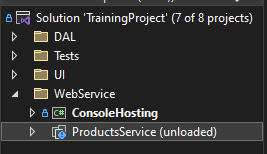
\includegraphics{screenshots/1.png}}
\label{fig:image}
\end{center}
Пробовал нажать Reload Project, но выдает ошибку
\begin{center}
\center{
\includegraphics{screenshots/2.png}}
\label{fig:image}
\end{center}
Попробовал сделать следующие шаги:\\
1 Remove the project from the solution.\\
2 Restart visual studio.\\
3 Add the project to the solution as an existing project.\\
Теперь такая ошибка
\begin{center}
\center{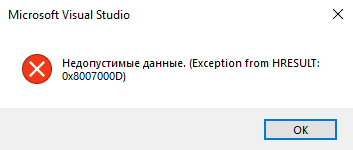
\includegraphics{screenshots/3.png}}
\label{fig:image}
\end{center}
Еще раз повторил действия, стала такая
\begin{center}
\center{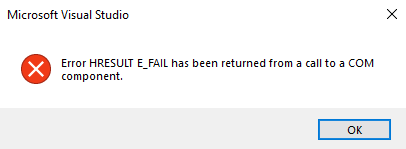
\includegraphics{screenshots/4.png}}
\label{fig:image}
\end{center}
Попробовал запустить WebService/ProductsService/ProductsService.csproj
\begin{center}
\center{
\includegraphics{screenshots/5.png}}
\label{fig:image}
\end{center}
Сделал следующие шаги, но не помогло
\begin{center}
\center{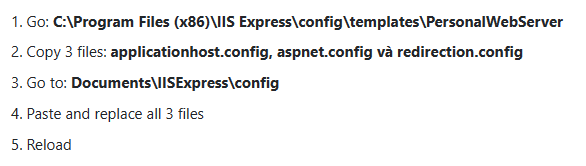
\includegraphics{screenshots/6.png}}
\label{fig:image}
\end{center}
\begin{center}
\center{
\includegraphics{screenshots/7.png}}
\label{fig:image}
\end{center}
Пробовал также множество других действий, но ничего к успеху не привело 
\end{document}








































